Nei diagrammi di sequenza viene illustrata l'interazione tra il \gloxy{server} ed i vari middleware, alcuni vengono forniti direttamente da Express mentre altri sono stati definiti dai \rPs. Un middleware può terminare la propria esecuzione in tre modi diversi:
\begin{enumerate}
\item Termina la propria esecuzione normalmente, eseguendo la richiesta passata dal middleware precedente, e quindi termina la catena;
\item Esegue la \gloxy{callback} passatagli come parametro, in questo modo passa il controllo ai successivi middleware;
\item Se si verifica un errore allora esegue la \gloxy{callback} passando come parametro l'errore verificatosi. In questo modo la \gloxy{callback} passerà il controllo al prossimo middleware della catena che è in grado di gestire l'errore.
\end{enumerate}
\subsubsection{Gestione generale delle richieste}\label{generReq}
Segue un elenco ordinato dei middleware utilizzati, l'ordine di elaborazione della richiesta è determinante poiché ciascuno costituisce un handler del \gloxy{design pattern} Chain of responsibility ed ha la facoltà di interrompere la catena del chiamante:
\begin{itemize}
\item \texttt{express.compress()}: middleware per comprimere con il formato gzip le comunicazioni;
\item \texttt{express.logger()}: middleware utilizzato per registrare un log delle richieste, utile per
fare il \gloxy{debugging} dell'applicazione;
\item \texttt{express.json()}: middleware che estrae dalla richiesta i parametri che sono nel formato
\gloxy{JSON};
\item \texttt{express.urlencoded()}: middleware che estrae dalla richiesta i parametri di tipo \texttt{www-form-encoded}, questi possono essere inviati ad esempio con una richiesta POST;
\item \texttt{express.methodOverride()}: middleware utilizzato per permettere anche ai vecchi \gloxy{browser} di avere un modo per fare richieste PUT e DELETE;
\item \texttt{express.cookieParser()}: middleware che analizza i cookie;
\item \texttt{express.cookieSession()}: middleware per la gestione di sessioni utente basate su cookies;
\item \texttt{passport.initialize()}: middleware per l’inizializzazione di Passport;
\item \texttt{passport.session()}: middleware che permette di memorizzare i record della sessione utente per mantenerne lo stato di login;
\item \texttt{express.route()}: permette di configurare un singolo route, nell'organizzazione interna di Premi::Back-End::App::Routers ogni modulo router contiene i routes logicamente correlati;
\item \texttt{AuthenticationController}: middleware scritto dai \rPs per gestire l’autenticazione. Utilizza nello specifico:
\begin{itemize}
\item \texttt{passport.authenticate()}.
\end{itemize}
\item \texttt{AuthorizationController}: middleware scritto dai \rPs per gestire tutte quelle operazioni che richiedono un livello di autorizzazione particolare oppure che operano su informazioni da verificare prima di essere passate al prossimo middleware. In particolare, il metodo \texttt{userById}, viene utilizzato come middleware a livello di router sul parametro id (relativo all'utente) per tutte le richieste che passano questo parametro;
\item \texttt{express.static()}: middleware per servire contenuti statici;
\item \texttt{NotFoundHandler}: un middleware scritto dai \rPs per gestire le richieste che non vengono gestite da nessun \gloxy{controller} (errore \gloxy{client} 404).
\item \texttt{ErrorHandler}: middleware scritto dai \rPs per gestire gli errori sollevati da altri middleware (errore \gloxy{server} 500).
\end{itemize}
Nel seguente diagramma di sequenza viene rappresentata una generica richiesta del \gloxy{client} al \gloxy{server}. Le classi ed il loro comportamento sono stati progettati in funzione del \gloxy{design pattern} Chain of responsibility che viene utilizzato internamente da Express (§\ref{Chain of responsibility}).
\begin{center}
\begin{figure}[h]
\centering
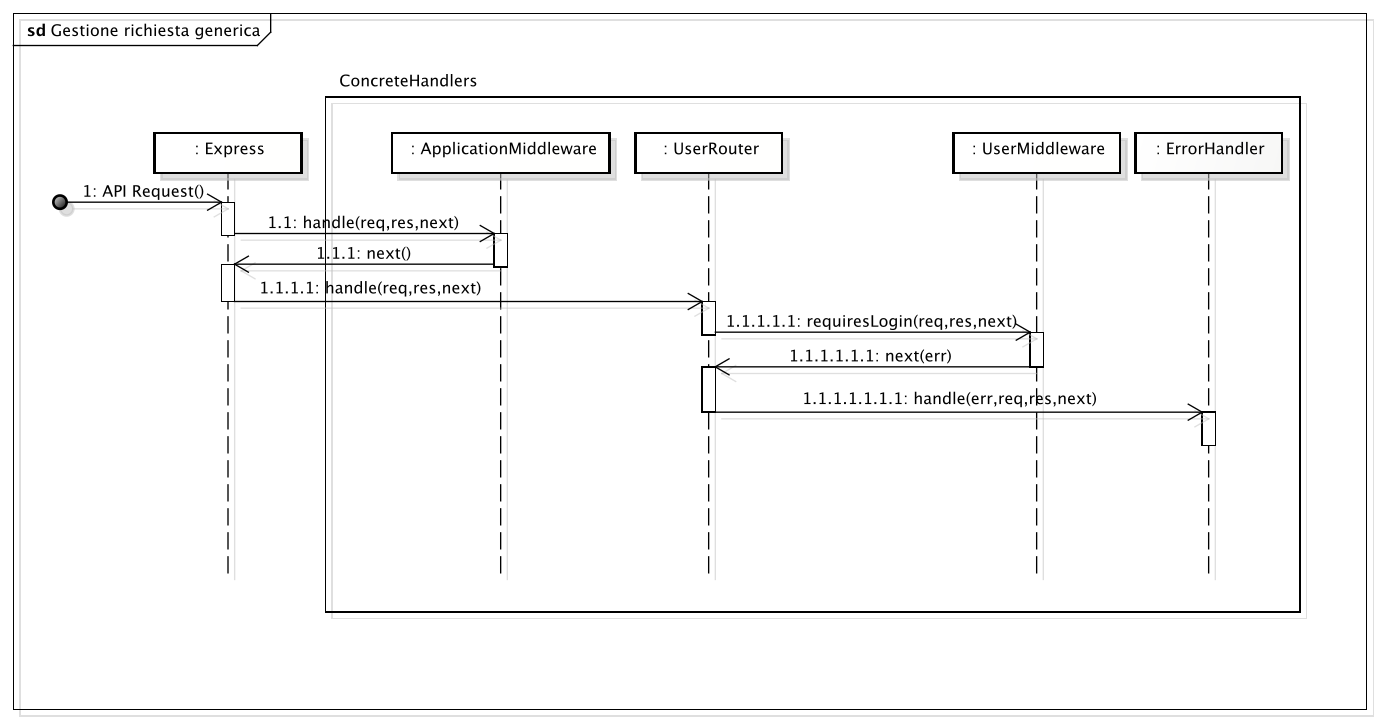
\includegraphics[scale=0.35,keepaspectratio]{diagrammi/sequenza/BackEnd/general.pdf}\label{figGeneral}
\caption{Gestione di una richiesta del client}
\end{figure}
\FloatBarrier
\end{center}
\subsubsection{Gestione dei fallimenti}
\subsubsubsection{Fallimento della procedura di registrazione}\label{regFailed}
Quando un utente effettua una richiesta di registrazione e cerca di inserisce dei dati già presenti nel database viene sollevato un errore.
Tale scenario rappresenta il fallimento di una richiesta di registrazione che impone, come vincolo per poter essere effettuata, che l'utente non sia autenticato e non possieda già un account nel sistema. In questo caso il modulo \texttt{AuthenticationController} invia \texttt{next(error)} per il fallimento di tale vincolo al router il quale avrà compito di reinstradarlo (indirizzandolo verso \texttt{ErrorHandler}).
\begin{center}
\begin{figure}[h]
\centering
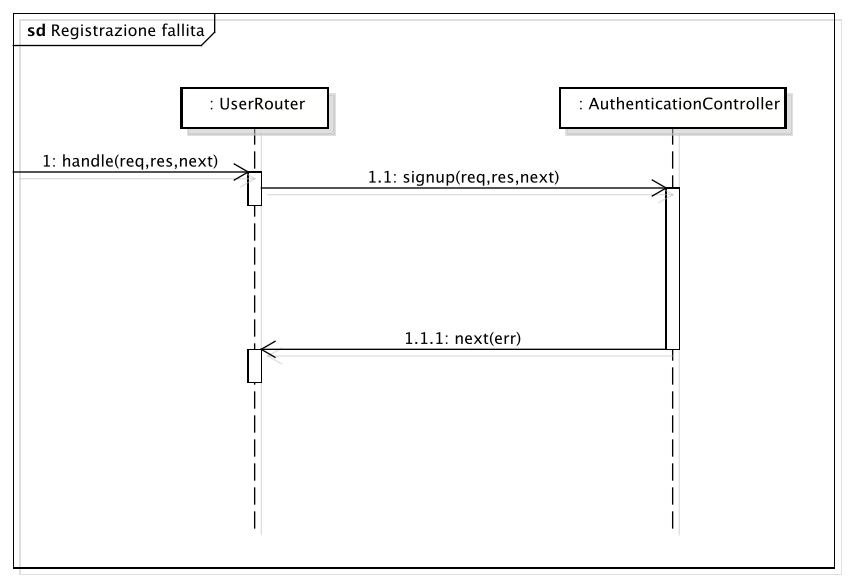
\includegraphics[scale=0.35,keepaspectratio]{diagrammi/sequenza/BackEnd/authFailed.pdf}
\caption{Fallimento della procedura di registrazione}
\end{figure}
\FloatBarrier
\end{center}
\subsubsubsection{Fallimento del vincolo "utente autenticato"}\label{userFailed}
La maggior parte delle richieste alle risorse rese disponibili dalle \gloxy{API} del \gloxy{server} possono essere effettuate solamente da un \emph{utente autenticato}. Tale scenario rappresenta il fallimento del vincolo ``utente autenticato''. La verifica del vincolo è gestita da \texttt{AuthorizationController} che invia \texttt{next(err)} a \texttt{UserRouter} che passerà successivamente il controllo alla catena di gestione degli errori.
\begin{center}
\begin{figure}[h]
\centering
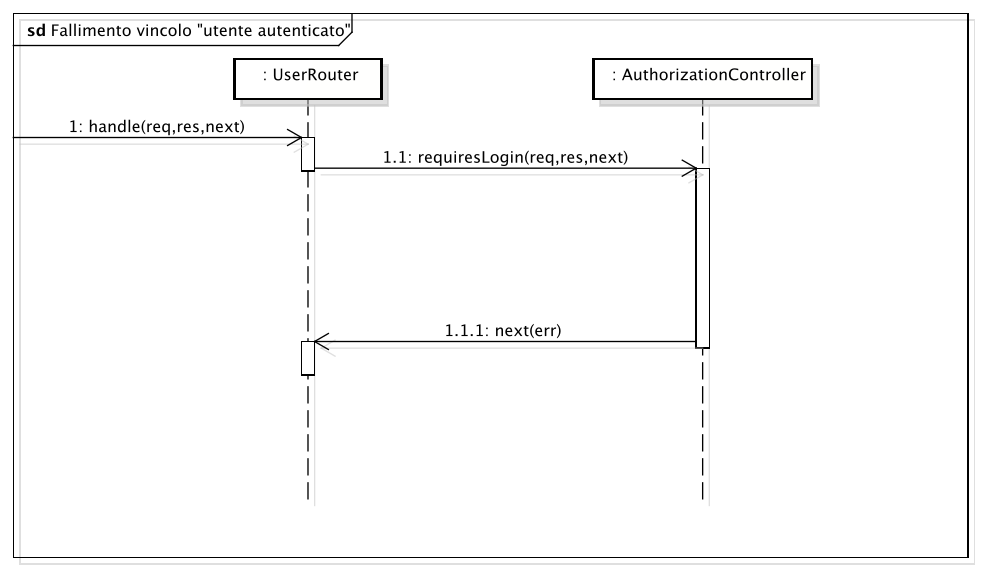
\includegraphics[scale=0.35,keepaspectratio]{diagrammi/sequenza/BackEnd/userFailed.pdf}
\caption{Fallimento del vincolo "utente autenticato"}
\end{figure}
\FloatBarrier
\end{center}
\subsubsubsection{Fallimento della richiesta di una lista di progetti}\label{projFailed}
L'utente autenticato può richiedere una lista di \gloxy{progetti} presenti nel database.  Nel caso in cui l'oggetto \texttt{req} sia \texttt{undefined} o malformato viene innescata la catena di gestione degli errori che ritornerà (attraverso l'oggetto \texttt{Response}) un messaggio d'errore specifico che verrà costruito dalla classe \texttt{PremiError}. Il controllo del programma, prima di passare a questo modulo, passerà ad \texttt{ErrorHandler}. Questo perché la classe \texttt{ErrorHandler} gestisce gli errori generici e qualora vi siano degli errori specifici legati al model viene invoca \texttt{next(err)} passando quindi il controllo a \texttt{PremiError}. Da notare inoltre che la classe \texttt{ProjectController} non compare nel diagramma di sequenza nonostante sia indicata nel diagramma relativo alle relazioni tra le classi del \gloxy{Back-End}. Questo perché la classe \texttt{ProjectController} serve per raggruppare tutti i controllers relativi al \gloxy{progetto} e quindi non espone alcun metodo suo (non ne ha) ma solamente i metodi dei controllers specifici del \gloxy{progetto}.
\begin{center}
\begin{figure}[h]
\centering
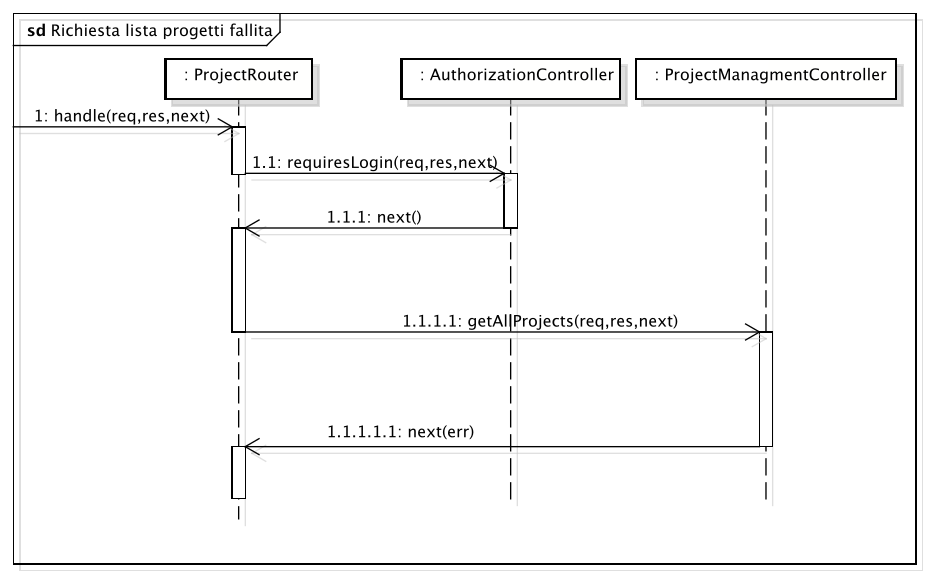
\includegraphics[scale=0.35,keepaspectratio]{diagrammi/sequenza/BackEnd/projFailed.pdf}
\caption{Fallimento della richiesta di un progetto}
\end{figure}
\FloatBarrier
\end{center}
\subsubsection{Richieste REST}
\subsubsubsection{DELETE /profile}\label{delProf}
\begin{center}
\begin{figure}[h]
\centering
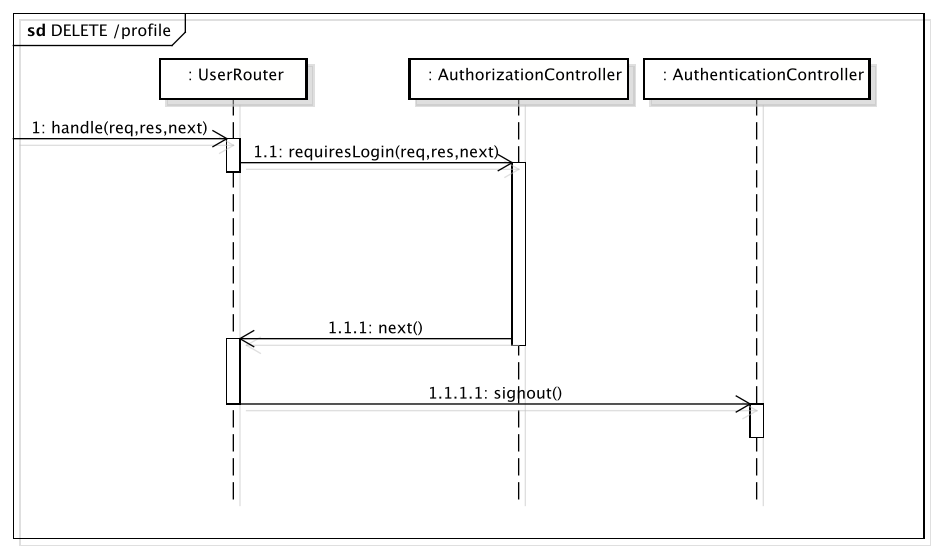
\includegraphics[scale=0.35,keepaspectratio]{diagrammi/sequenza/BackEnd/delProf.pdf}
\caption{DELETE /profile}
\end{figure}
\FloatBarrier
\end{center}
\subsubsubsection{DELETE /projects/:projectId}\label{delProj}
\begin{center}
\begin{figure}[h]
\centering
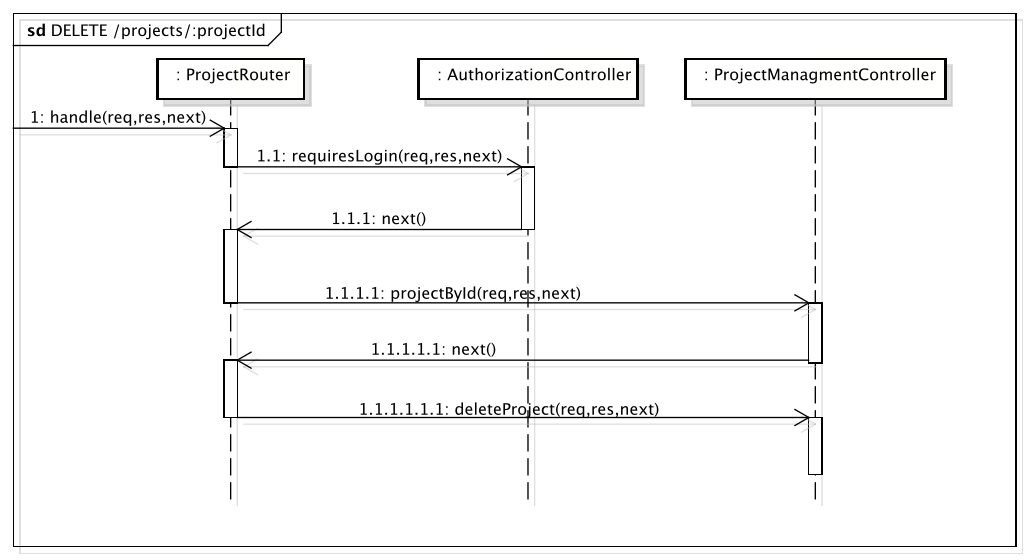
\includegraphics[scale=0.35,keepaspectratio]{diagrammi/sequenza/BackEnd/delProj.pdf}
\caption{DELETE /projects/:projectId}
\end{figure}
\FloatBarrier
\end{center}
\subsubsubsection{PUT  /projects/:projectId}\label{putProj}
\begin{center}
\begin{figure}[h]
\centering
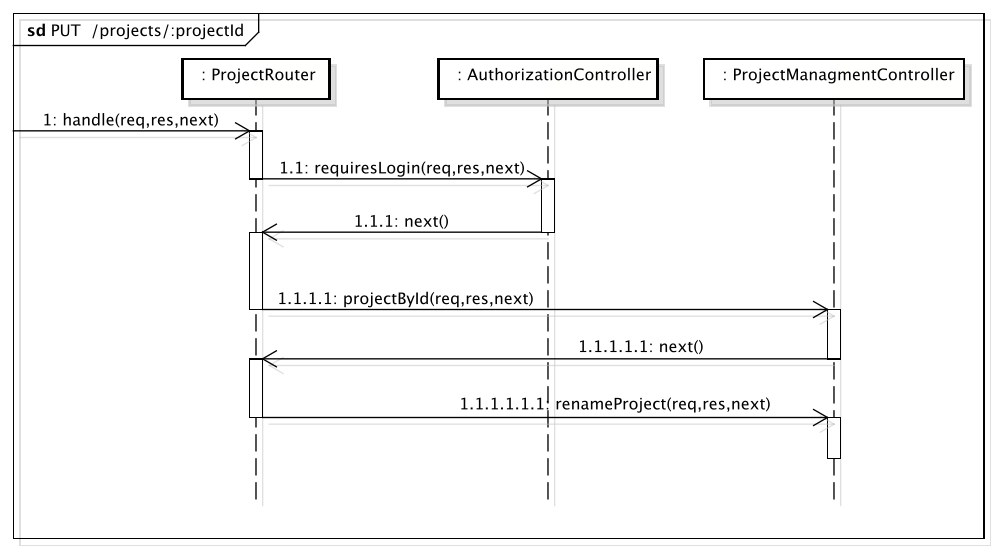
\includegraphics[scale=0.35,keepaspectratio]{diagrammi/sequenza/BackEnd/putProj.pdf}
\caption{PUT  /projects/:projectId}
\end{figure}
\FloatBarrier
\end{center}
\subsubsubsection{GET  /projects/:projectId}\label{getProj}
\begin{center}
\begin{figure}[h]
\centering
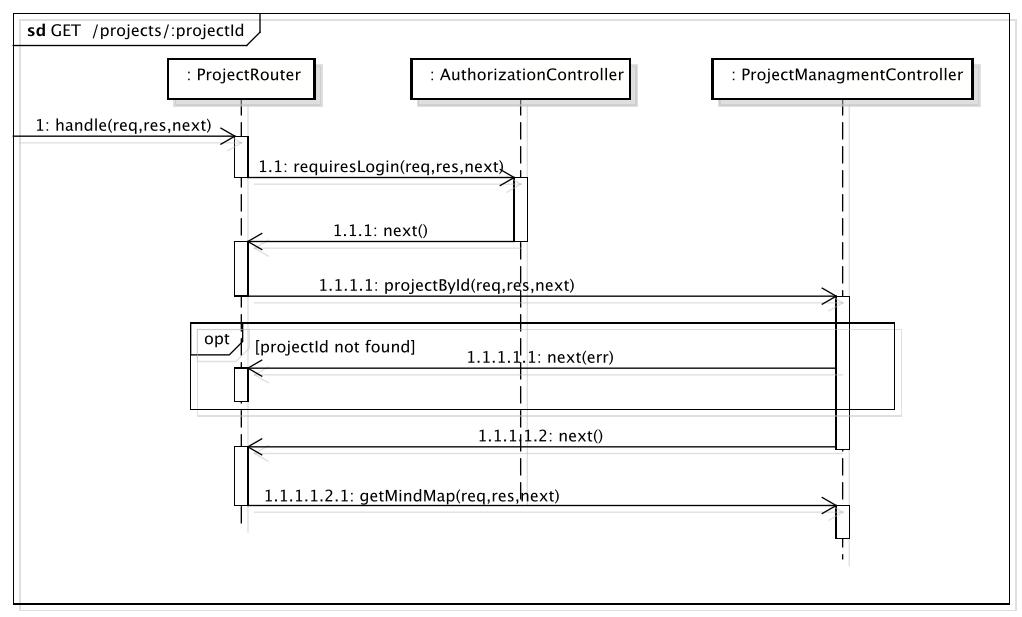
\includegraphics[scale=0.35,keepaspectratio]{diagrammi/sequenza/BackEnd/getProj.pdf}
\caption{GET  /projects/:projectId}
\end{figure}
\FloatBarrier
\end{center}
\subsubsubsection{PUT  /projects/:projectId/nodes/:nodeId}\label{putNod}
\begin{center}
\begin{figure}[h]
\centering
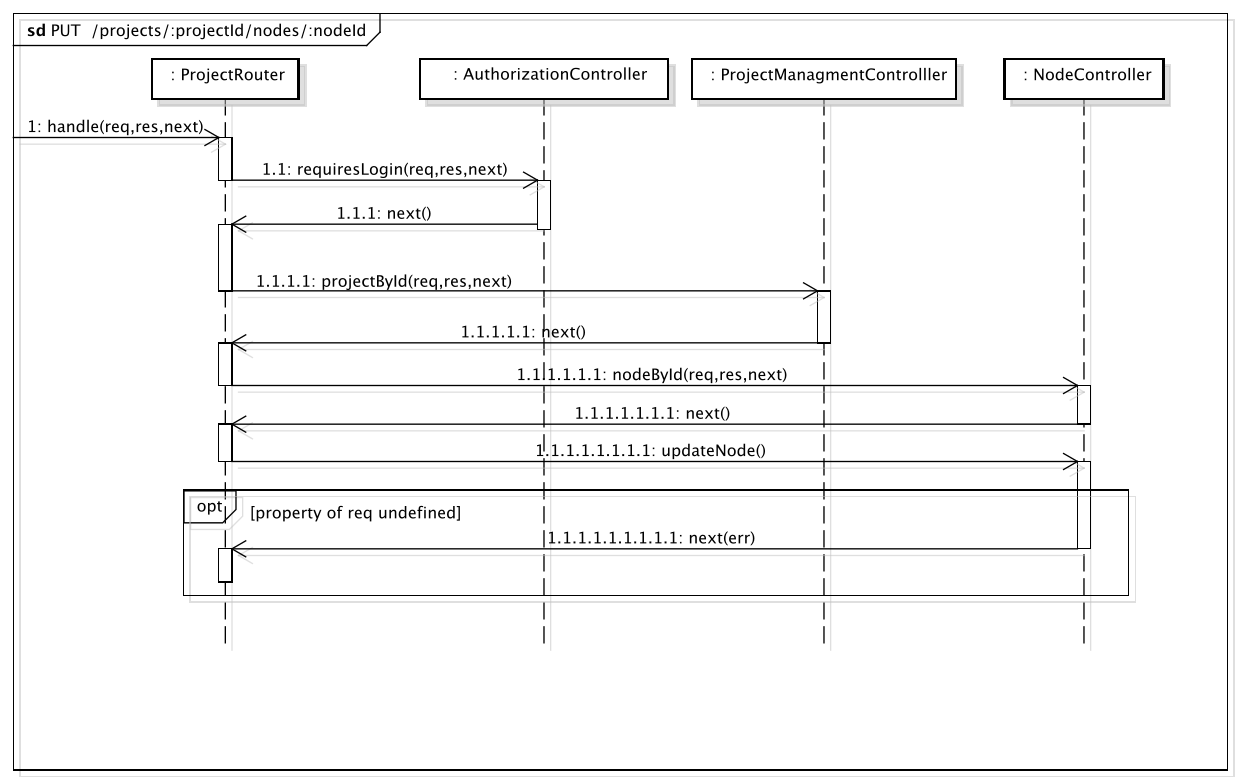
\includegraphics[scale=0.35,keepaspectratio]{diagrammi/sequenza/BackEnd/putNod.pdf}
\caption{PUT  /projects/:projectId/nodes/:nodeId}
\end{figure}
\FloatBarrier
\end{center}
\subsubsubsection{POST  /projects/:projectId/associations}\label{postAss}
\begin{center}
\begin{figure}[h]
\centering
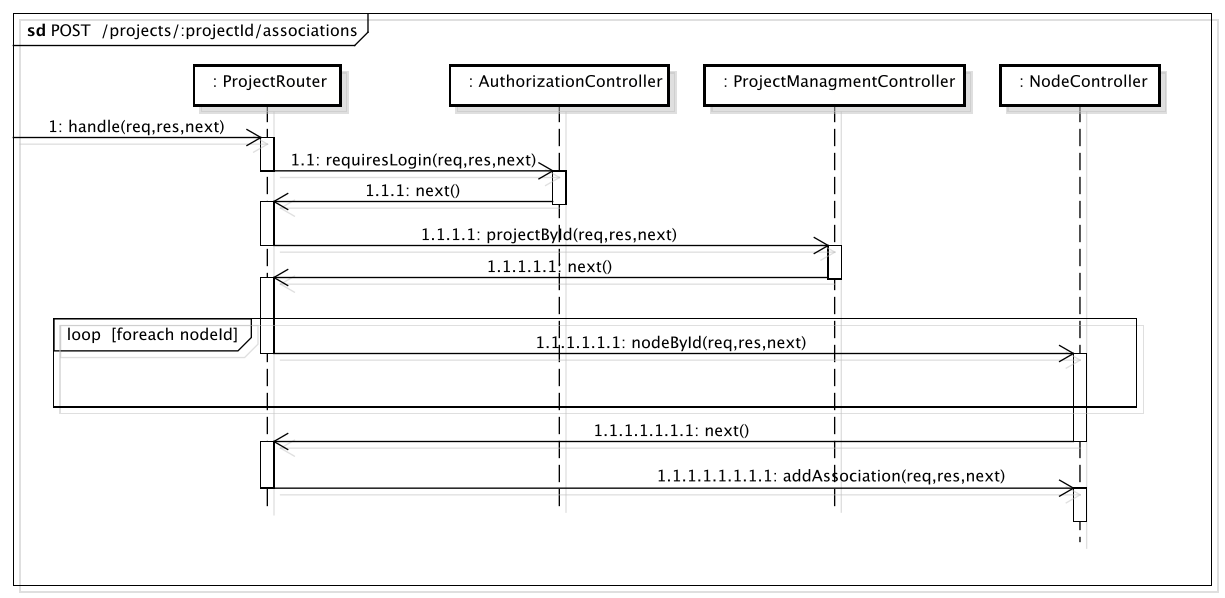
\includegraphics[scale=0.35,keepaspectratio]{diagrammi/sequenza/BackEnd/postAss.pdf}
\caption{POST  /projects/:projectId/associations}
\end{figure}
\FloatBarrier
\end{center}
\subsubsubsection{DELETE  /projects/:projectId/associations/:associationId}\label{delAss}
\begin{center}
\begin{figure}[h]
\centering
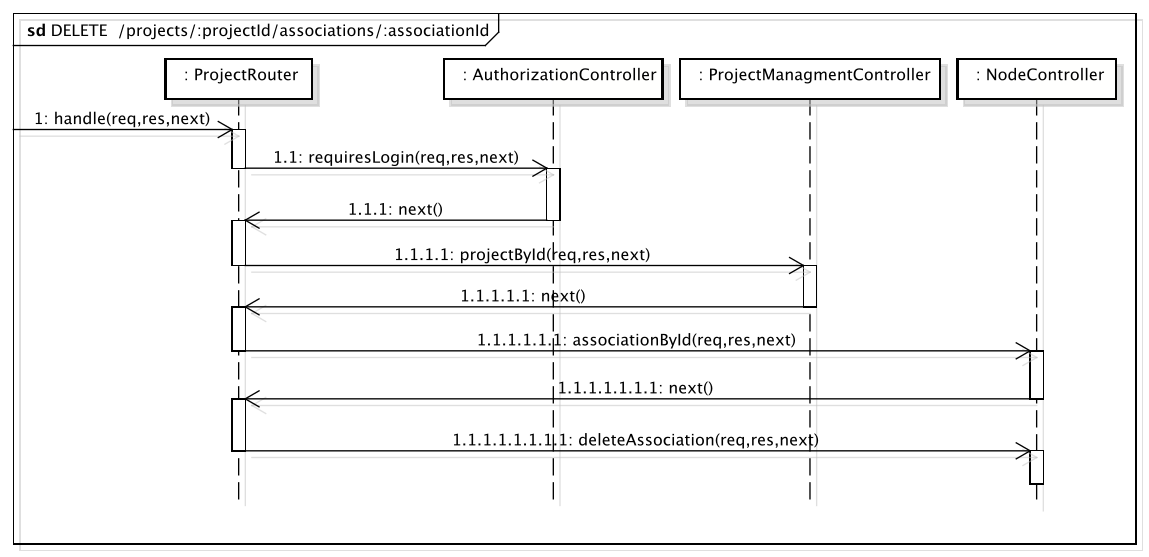
\includegraphics[scale=0.35,keepaspectratio]{diagrammi/sequenza/BackEnd/delAss.pdf}
\caption{DELETE  /projects/:projectId/associations/:associationId}
\end{figure}
\FloatBarrier
\end{center}
\subsubsubsection{PUT  /projects/:projectId/path/:pathId}\label{putPath}
\begin{center}
\begin{figure}[h]
\centering
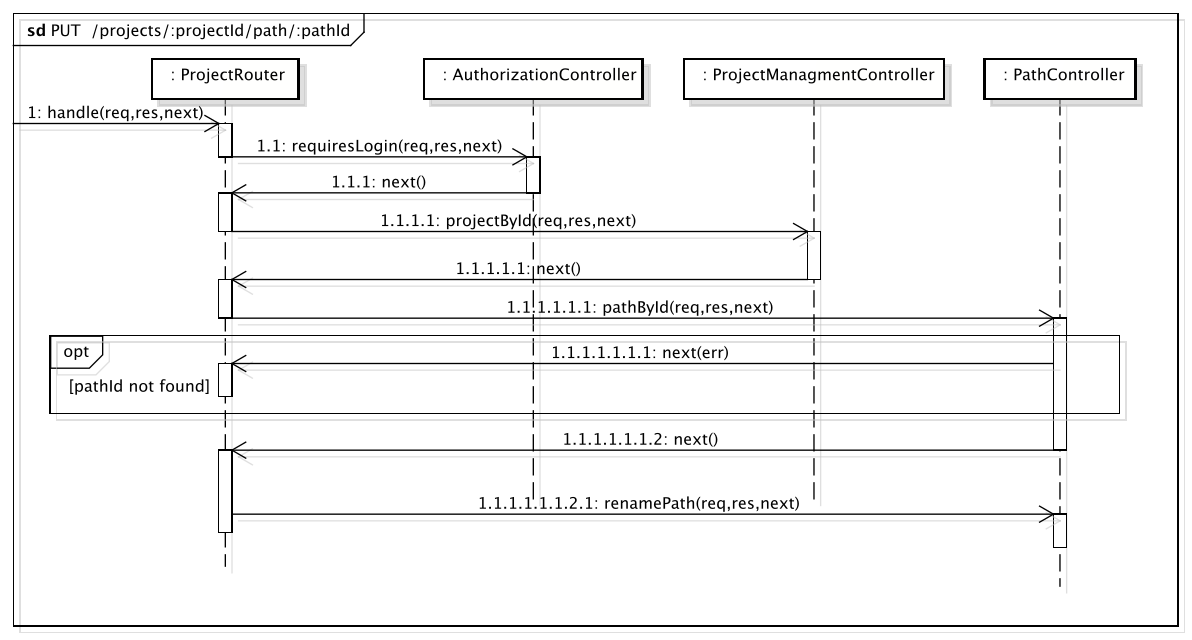
\includegraphics[scale=0.35,keepaspectratio]{diagrammi/sequenza/BackEnd/putPath.pdf}
\caption{PUT  /projects/:projectId/path/:pathId}
\end{figure}
\FloatBarrier
\end{center}
\subsubsubsection{POST  /projects/:projectId/path/:pathId}\label{postPath}
\begin{center}
\begin{figure}[h]
\centering
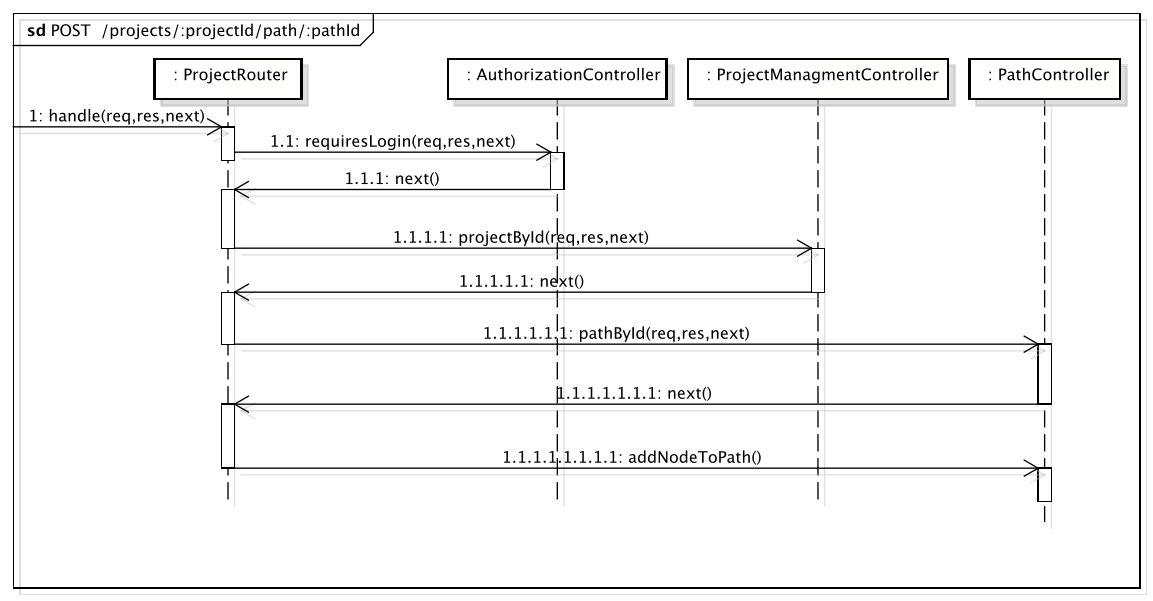
\includegraphics[scale=0.35,keepaspectratio]{diagrammi/sequenza/BackEnd/postPath.pdf}
\caption{POST  /projects/:projectId/path/:pathId}
\end{figure}
\FloatBarrier
\end{center}
\subsubsubsection{GET  /projects/:projectId/premiPresentation}\label{getPremi}
\begin{center}
\begin{figure}[h]
\centering
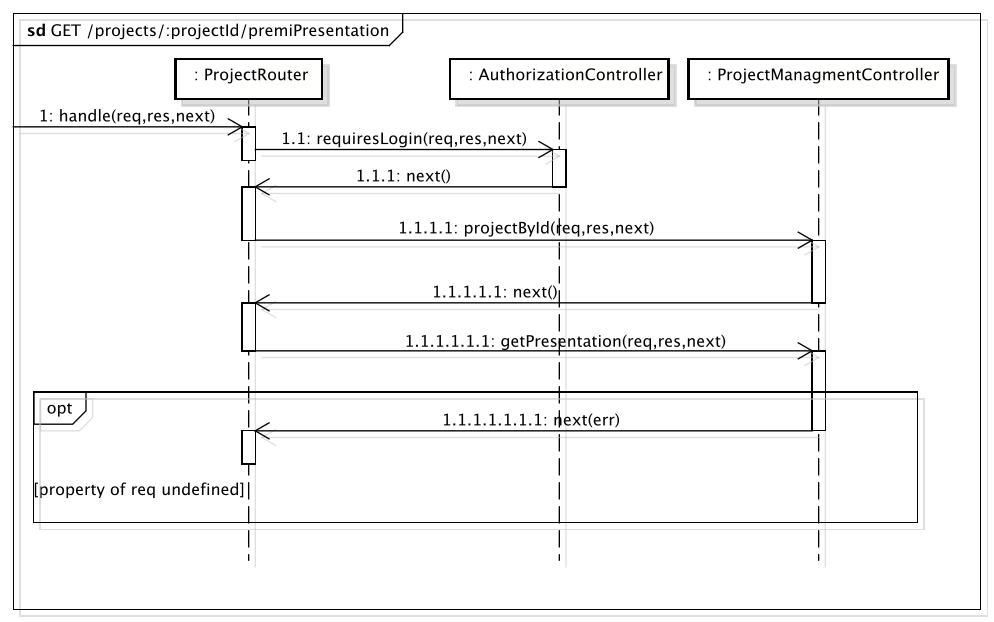
\includegraphics[scale=0.35,keepaspectratio]{diagrammi/sequenza/BackEnd/getPremi.pdf}
\caption{GET  /projects/:projectId/premiPresentation}
\end{figure}
\FloatBarrier
\end{center}
\subsubsubsection{GET  /static/userManual}\label{getStat}
\begin{center}
\begin{figure}[h]
\centering
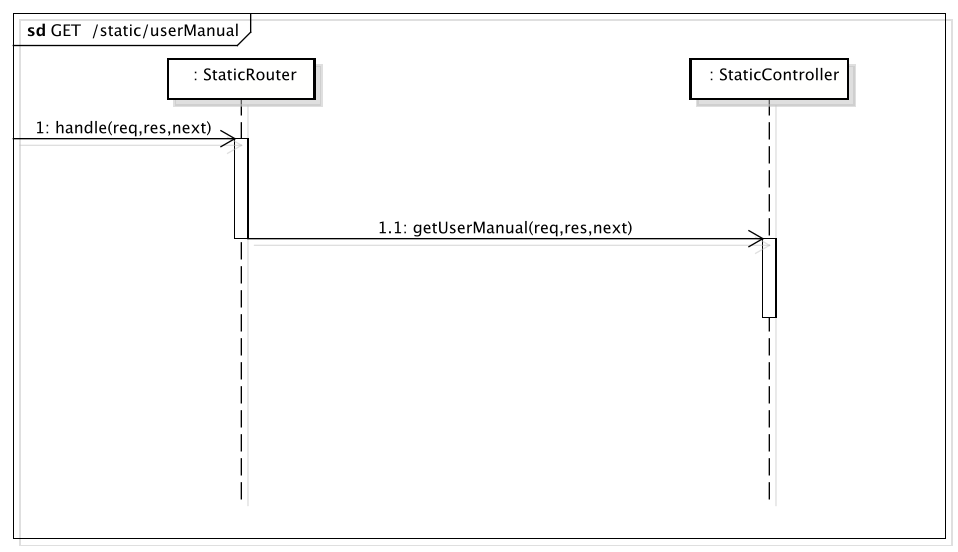
\includegraphics[scale=0.35,keepaspectratio]{diagrammi/sequenza/BackEnd/getStat.pdf}
\caption{GET  /static/userManual}
\end{figure}
\FloatBarrier
\end{center}
